What is the relationship between a Transnational Entrepreneur's network and their knowledge diffusion within the context of the Berlin Startup sphere.
%%%%%%%%%%%%%%%%%%%%%%%%%%%%%%%%%%%%%%%%%%%%%%%%%%%%%%%%%%%%%%%%%%%%%%%%%%%%%%%%
\section{The Theoretical Model}
%%%%%%%%%%%%%%%%%%%%%%%%%%%%%%%%%%%%%%%%%%%%%%%%%%%%%%%%%%%%%%%%%%%%%%%%%%%%%%%%
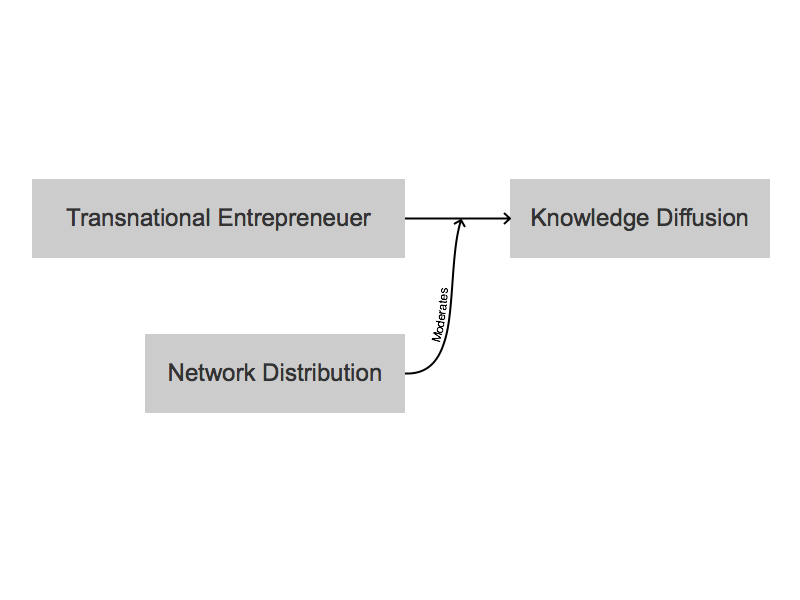
\includegraphics[width=1.0\textwidth]{theoretical_model.png}
The database structure was designed to be as simple and extensible as possible. There are three tables, 'edge', 'node', and 'status'. As you may imagine, the 'edge' table stores all relationships between 'node' objects, the 'node' table stores all nodes, and the 'status' table stores all statuses.
\subsection{The Relationships}
The Declarative Base is a special feature of SQLAlchemy. By extending the base class and providing some protected members with metadata, we are able to create a table of a given type in SQLAlchemy. In the example below, we have created a class Node that extends Base. For our metadata we have provided \verb|__tablename__| which indicates what the table name within our database will be. Additionally we have defined all of the fields and their types which will automatically be instantiated by SQLAlchemy when the engine is created. Additionally you'll see that we have a one:many relationship defined between a given Node and a set of Statuses. That is, a Node can have multiple Statuses (this represents all of the tweets made by the user).

